\question{Дифференциальное уравнение поступательного движения частицы сплошной
среды. Ковариантная форма уравнения движения. Движение частицы сплошной
среды относительно ее центра масс. Закон парности касательных напряжении.}

Воспользуемся теоремой о движении центра масс системы частиц и применим её к
частице сплошной среды массой \( m \) - ускорение центра масс \( \vec{a} \)
определяется суммой внешних по отношению к системе сил:
\[
    m\vec{a} = \sum \vec{F}_i^e.
\]

Силы действующие со стороны других тел называют объёмными (в отсутствие
электромагнитных полей -- массовыми). Массовые силы пропорциональны массе
частицы среды:
\[
    F^i = \rho_m V f^i,
\]
где \( f^i \) -- вектор напряжённости, \( \rho_m  \) -- плотность. Электрические
силы пропорциональны заряду частицы среды:
\[
    F^i = \rho_e V E^i
\]

Силы, действующие со стороны частиц среды называют \emph{поверхностными}.
Поверхностные силы не определяют в аналитическом виде. Вместо этого вводят
понятие \emph{тензора напряжений} \( \sigma^{ji} \).

\sidefig(9cm)
{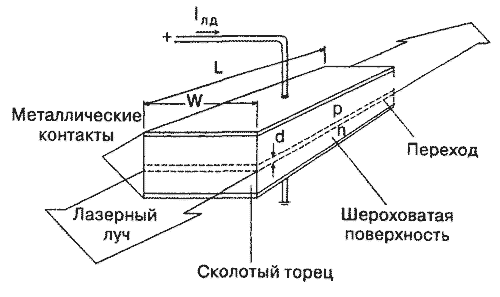
\includegraphics[width=\textwidth]{30_01}}{
Рассмотрим малый объём сплошной среды, разделим его на две части, как показано
на рисунке, и отбросим половину частицы. Силы действующие на частицу со стороны
отброшенной части \( dF^j \) пропорциональны площади, точнее, если ввести
ковариантный вектор \( dS_i \), нормальный к элементу поверхности: 
\[
    dF^j = \sigma^{ji} dS_i.
\]
}

Тогда \( F^j \), действующая на частицу со стороны поверхностных сил,
определится в виде:
\[
    F^j = 
    \oint\limits_S dF^j = 
    \oint\limits_S \sigma^{ji} dS_i =
    \oint\limits_S \int\limits_{x_{i0}}^{x_{i1}} \pder{\sigma^{ji}}{x^i} dx^i
    dS^i =
    \int\limits_V \pder{\sigma^{ji}}{x^i} dV =
    \int\limits_V \nabla_i \sigma^{ji} dV.
\]
    
Считая, что объём \( V \) частицы мал:
\begin{gather*}
    \rho V \frac{\delta v^i}{dt} = \rho V f^i + \nabla_j \sigma^{ij} V,\\
    \rho \frac{\delta v^i}{dt} = \rho f^i + \nabla_j \sigma^{ij}, \\
    \rho \left( \der{v^i}{t} + v^k \Gamma^i_{kj} v^j\right) = \rho f^i +
    \nabla_j \sigma^{ij}.
\end{gather*}

Последнее уравнение и является уравнением поступательного движения частицы
сплошной среды в ковариантной форме. В декартовых координатах:
\begin{gather*}
    \rho  \der{v^i}{t}  = \rho f^i + \pder{ \sigma^{ij}}{x^j}.
\end{gather*}

\sidefig(9cm)
{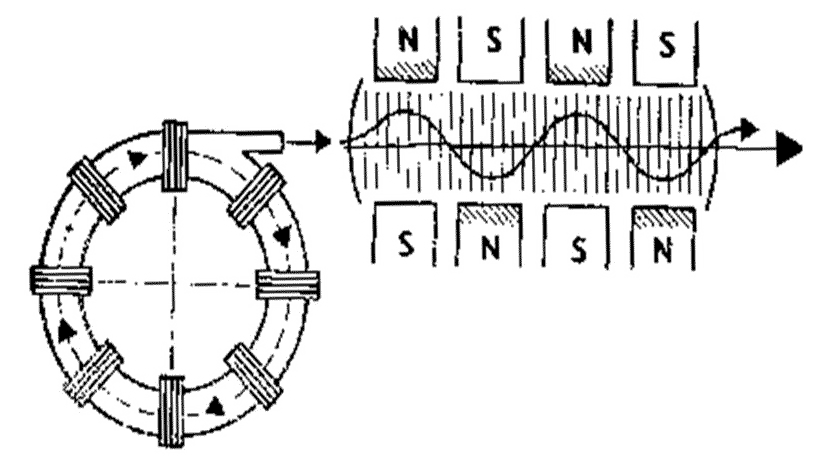
\includegraphics[width=\textwidth]{30_02}}{  
Рассмотрим движение частицы (в виде малого куба с центром масс в центре, как на
рисунке) вокруг центра масс. По теореме об изменении момента количества
движения \( K \) относительно оси \( p \), изображённой на рисунке, проведённой
через центр масс \( C \):
\[
    \der{K}{t} = \sum M^e.
\]
}

Силы действующие на куб со стороны боковых граней и создающие моменты \( M^e \):
\( \sigma^{13}dS_3 \), \( -\sigma^{13}dS_3 \), \( \sigma^{31}dS_1 \),
\( -\sigma^{31}dS_1 \), считая что сторона куба \( \delta h \), получим:
\[
    \der{K}{t} = -2\sigma^{13}\delta h^3+ 2\sigma^{31}\delta h^3.
\]

Но \(K \sim m \delta h^2 \sim \delta h^5\) и слева стоит величина более
высокого порядка малости, чем справа. И теорема об изменении момента количества
движения относительно оси \(p\)
\[
    \sigma^{31} = \sigma^{13}.
\]

Аналогично можно получить ещё два соотношения, вместе они выражают уравнения
сферического движения частицы сплошной среды:
\[
    \sigma^{ij} = \sigma^{ji}.
\]

Это соотношение носит название \emph{закона парности касательных напряжений}. 

\newpage
